\chapter{Architektur}

\section{Prämisse}
Im Aufbau des Projekts wird das Konzept der "`Clean Architecture"' umgesetzt \cite{CleanArchitecture} \cite{AndroidGuidelines}. Das bedeutet, dass eine klare Modularisierung besteht. Kernfunktionen und Geschäftslogik werden von der Benutzeroberfläche, sowie von den Datenquellen getrennt. Somit sind die einzelnen Komponenten der Architektur leicht austauschbar. 
Die Grafik \ref{cleanarch} zeigt dieses Prinzip. Die grundlegenden Strukturelemente des Projekts liegt in "`Entity"'. In "`Use Case"' ist die Funktionalität der Entities enthalten.  Im oberen Teil des äußeren Rings ist die direkte Benutzeroberfläche, in der Eingaben verarbeitet werden, sowie die Abstraktion "`Presenter"', welche Logik zum Verarbeiten der Nutzereingaben stellt, zu sehen. Im unteren Teil bietet"`Repository"' eine Schnittstelle zu den verschiedenen Datenquellen, welche - genau wie "`UI"' - reale Einrichtungen (z.B. Datenbanken und Webserver) darstellen.
Dabei ist zu beachten, dass sich Abhängigkeiten einer äußeren Schicht nur auf innere Schicht beziehen dürfen, was anhand der unausgefüllten Pfeile sichtbar ist. Innere Schichten dürfen also keinerlei Wissen von Aufbau und Funktionalität von höher liegenden Schichten haben. Der Kern "`Entity"' hat demnach keine Abhängigkeiten. Dies ist das Prinzip der {\em Dependency Inversion}.
Der Datenfluss fließt trotz der Abhängigkeits-Regel bidirektional durch alle Schichten hindurch, da z.B. Daten, die aus einer Datenquelle geladen werden, auch in der Oberfläche sichtbar gemacht und dort ggf. auch geändert werden. Dies ist durch gewisse Entwurfsentscheidungen möglich, auf die in späteren Kapiteln noch näher eingegangen wird.


%Bsp-Grafik CleanArchitecture
\begin{figure}[H]
\centering
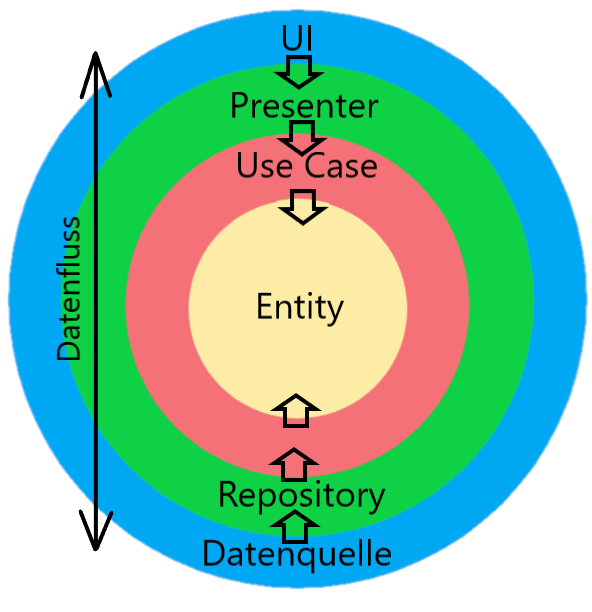
\includegraphics[width=0.51\textwidth]{pics/cleanArchitecture.png}%
\caption{Clean Architecture Prinzip grafisch dargestellt}%
\label{cleanarch}%
\end{figure}

\section{App}


\subsection{Layered Architecture}

Wenn man sich die konzentrischen Ringe von Robert C. Martins Clean Architecture einmal vertikal aufgeschnitten vorstellt, sieht man gut, dass die Clean Architecture zu einer Schichtenarchitektur führt, die den Code klar strukturiert.


\begin{itemize}
\item {\textbf{User Interface Layer}} (UI und Presenter)
\item {\textbf{Domain Layer}}  (Use Cases und Entities)
\item und {\textbf{Data Layer}}. (Repository, Datenquelle)
\end{itemize}


%Bsp-Grafik  Layer
\begin{figure}[H]
\centering
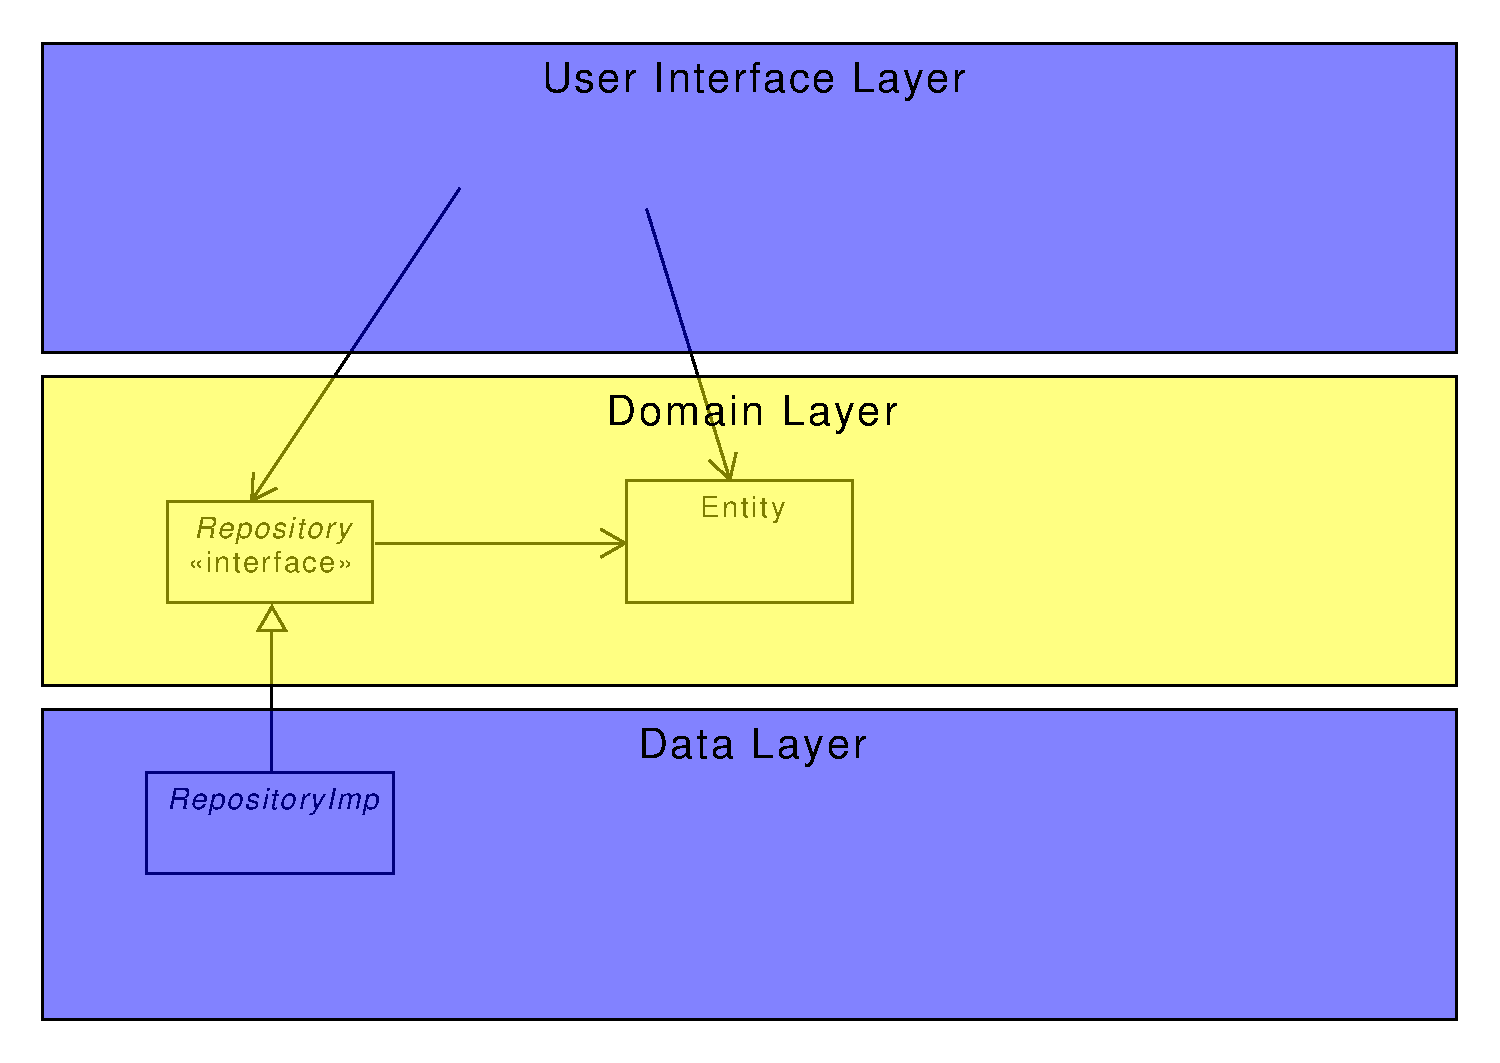
\includegraphics[width=0.5\textwidth]{pics/layers.pdf}%
\caption{Layer mit Dependency Inversion}%
\label{cleanarch}%
\end{figure}

\subsection{Domain Layer} 
Im Kern der Architektur steht die {\em Business Entities}, die unsere Domäne modellieren.
Diese beschreiben die "`realen"' Objekte unserer Domäne und die Methoden, die mit ihnen möglich sind. Genauer gesagt also Entitäten, wie zB. Rezepte, die es auch gäbe, wenn man das Kochbuch in Papierform führen würde. 

%Todo Glossarreferenz Clean Architekture Chapter 20 Business Rules

In diesem Entwurf ist das sogenannte "`Domain Driven Design"' umgesetzt \cite{CleanArchitecture} \cite{DomainDrivenDesign}, das heißt, dass die Kernentitäten szenariobasiert ermittelt wurden. Somit sind sie aus Szenariensicht von der Domäne aus und nicht von der Datenbank her modelliert.


\subsubsection{Repository-Schnittstelle}
Zusätzlich zu den Entitäten gehört zu dem innersten Kern der Clean Architecture die Repositoryschnittstelle für die einzelnen Entities.

Diese Schnittstelle kapselt, die durch die Datenzugriffsschicht persistierten Objekte und den Zugriff auf sie, unabhängig davon, ob sie lokal in der Datenbank gespeichert oder per Webservice zur Verfügung gestellt werden. 
Die Repository-Schnittstelle ist dabei als Schnittstelle (abstrakte Klasse) modelliert und stellt aus Sicht der Domain Logik, die nötigen Speicherfunktionen und Suchfunktionen, die die Anwendung braucht, dar. 

%Todo Referenz auf Repository Entwurfsmuster
%https://de.wikipedia.org/wiki/Repository_(Entwurfsmuster)
%Martin Fowler Patterns fo Enterprise Appplication 
%LI


\subsection{Data Layer} 
Die Datenschicht implementiert die Repositoryschnittstelle. Konzeptionell verhält sich das Repository aus Schnittstellensicht, wie eine Liste von Fachobjekten mit den bereitgestellten Methoden zum Laden und Speichern neuer Elemente.

In der Datenschicht wird zum einen die Persistierung in der lokalen SQLite Datenbank mit den in Android Bibliothek {\em Room} und zum anderen das Laden und Speichern der Objekte über die REST-Schnittstelle des Servers mit {\em Retrofit} umgesetzt. Die Bibliotheken sind von Google in den Android Jetpack Developer Guides empfohlen und werden deswegen eingebunden.

Jedes Repository wird mithilfe von DAOs (Data Access Objects) implementiert, die den Zugriff auf einzelne Tabellen in der Datenbank mit der relationalen Datenbanklogik zum Laden und Speichern kapseln. 

%\subsubsection{Dependency Inversion} 
%Was hier beschrieben ist, ist das Prinzip der {\em Dependency Inversion} 
%das Data Layer implementiert die abstrakten Repository Schnittstellen. 
%Dadurch wird genau die im Cleanarchitekturediagramm geforderte Abhängigkeit erreicht. Die Datenzugriffschicht hängt von dem Domain Layer ab
%und nicht umgekehrt. 

\subsection{UserInterface Layer}

\subsubsection{MVVM} 
Als Grundgerüst für die Strukturierung des User Interface Layer wird das Model-View-ViewModel (MVVM) Entwurfsmuster verwendet. 
Dabei beinhaltet "`View"' die grafische Benutzeroberfläche, sowie Anweisungen, wie auf Nutzer- und App Eingaben reagiert werden soll. 

Das "`ViewModel"' (VM) überwacht die View. Werden durch App-Interaktionen Daten in der View angefordert oder verändert, so merkt das VM dies und gibt dem Model die entsprechenden Befehle weiter. Es ist also ein Vermittler zwischen View und Model.
Durch die im Domain Layer beschriebenen Repositoryschnittstelle laden und speichern die ViewModellklassen Fachobjekte. 
%TODO Glossareintrag Fachobjekte

%Todo auf Fabrikmuster bezug nehmen. 
Das "`Model"' in MVVM steht für die Logik der grundlegenden App Funktionen. Im Falle von Exzellenzkoch sind das genau die Entityklassen und Repositoryschnittstellen, wie sie im Domain Layer definiert werden. 


\subsection{Zusammenfassung}
Ein Ziel dieser Architektur ist die Entkoppelung der sich ändern könnenden Schichten. So sind z.B. Nutzerschnittstelle und Datenschicht nur ein Detail. 

Die Anwendung wird so aufgebaut, dass zum Beispiel eine völlig andere Nutzerschnittstelle statt der Androidapp, oder ein dateibasierter Speicher statt einer relationalen Datenbank, umsetzbar wäre, ohne, dass dies auf die anderen Schichten Einfluss hätte.

Ein Vorteil, der dadurch entsteht, ist die klare Abgrenzung der einzelnen Funktionen und die leichtere Testbarkeit und Wartbarkeit der einzelnen Subsysteme. Außerdem wird durch diese Modularisierung das ganze Projekt leicht erweiterbar gemacht.

\section{Server}

\subsection{Einleitung}
Registriert sich ein Nutzer in der App, so kann er mit anderen Nutzer interagieren. Diese Interaktion wird durch die Serverkomponente ermöglicht. Ein eingeloggter User, kann mit der App auf seinem Smartphone Daten zum Server schicken und damit zum Beispiel Rezepte veröffentlichen. Andere eingeloggte User können dann nach diesen Rezepten suchen. 
Um dies zu ermöglichen, bietet der Server eine REST-Schnittstelle an. 
Unter verschiedenen "`Endpoints"' werden, ähnlich wie bei der Repositoryschnittstelle, verschiedene Methoden angeboten, um Entities zu laden und zu speichern. 

\subsubsection{Beispiel}
Ein HTTP GET auf den Endpunkt:

http://psekochbuch.de/api/users/MagnumMandel\footnote{Dies ist nur ein grober Überblick, modulo Authentifizierung. Ist diese aktiviert, erfolgt die Verbindung TLS-verschlüsselt. Gegebenenfalls leitet der Resource Server (unser Server) einen nicht authorisierten User an den Authentication Server von Google weiter, und erst wenn dieser mit korrektem JSON-Access-Token anfragt wird das JSON-Dokument als Antwort geschickt}


liefert zum Beispiel das passende JSON-Dokument zurück:
\begin{lstlisting}
{
  "userid": "MagnumMandel",
  ...
  "description": "Veganer essen meinem Essen das Essen weg."
}

\end{lstlisting}


Im Folgenden wird der Server mit seinen Komponenten näher beschrieben. 

\subsection{Technologiestack}
Der Server wird als Spring-Boot-Anwendung mit Rest-Schnittstelle umgesetzt.
Authentifizierung erfolgt nach dem OAuth 2.0 Standard mit JSON-Webtokens und soll mit Hilfe der Firebase Library verwirklicht werden. Die Daten werden mit Hilfe von Hibernate auf eine relationale Datenbank gemappt und gespeichert und geladen. 

\subsection{Struktur} 
Spring-Boot hat mit integrierter Dependency-injection und Annotationen einen klare Vorgabe, wie eine REST-Applikation umzusetzen ist. Mit verschiedenen Annotationen werden Klassen ausgezeichnet. Diese annotierten Klassen, die das Grundgerüst der Anwendung darstellen, werden Beans genannt. Der Spring IOC Container assembliert diese Beans dann, gemäß ihrer durch Annotationen bestimmten Rollen, zu einer Anwendung. 

\begin{figure}[H]
\centering
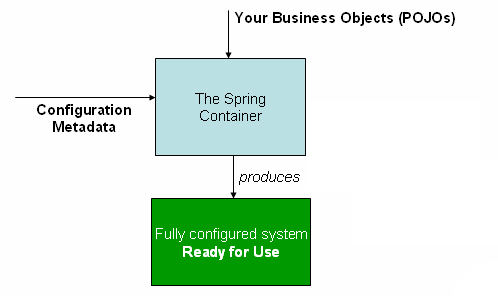
\includegraphics[width=0.6\textwidth]{pics/spring_ioc_container.png}%
\caption{Spring Inversion of Control Container\cite{SpringCoreTechnologies}}%
\label{cleanarch}%
\end{figure}

Der Server ist in verschiedene Bereiche aufgeteilt: \\
Zum einen gibt es eine Klasse, die die Einstellungen für den Server und die Logik für die Authentifizierung,  wie z.B. die Verbindung zu einer Authentifizierungsschnittstelle wie Firebase und die Überprüfung des JSON-Tokens,  beinhaltet. \\
Des weiteren gibt der Server eine API an, durch welche die Restschnittstelle mit ihren Endpunkten definiert wird. \\
Ein weiterer Bereich enthält die Logik für die Datenhaltung und Ansteuerung dieser API. \\

Die Paketeinteilung ist in Kapitel 4.2 erläutert. 
\section{Deployment}
 
\subsection{Server-Deployment} 
Als Springboot-Applikation ist die deploybare App des Servers ein JAR-File, dass den HTTP-Server Tomcat und alle Abhängigkeiten enthält. Es braucht kein vollwertigen Java EE Server konfiguriert und installiert werden, der dann einem WAR oder EAR bestückt. Das heißt als Umgebung auf unserem Bw-Cloud-server wird nur ein Linuxsystem mit installiertem JavaJDK und eine relationale Datenbank benötigt. 

\subsection{App-Deployment}
Das Gradle Build-tool erstellt eine apk-Datei, die alle benötigten Bibliotheken, die nicht auf den Endgeräten vorausgesetzt werden und das Manifest, was die Installation spezifiziert, enthält. Die apk-Datei kann dann entweder über das Android Debug Bridge-Tool (adb) direkt auf ein Endgerät installiert oder über den {\em Google Play Marketplace} veröffentlicht werden.


\section{Authentifizierung und Authorisierung} 
Die App und der Server sollen ein Rechtemodell umsetzen. 
Das bedeutet, dass Nutzer, je nach Status, unterschiedliche Rechte für die Nutzung der Funktionalität der App, besitzen. Beispielsweise soll jeder Nutzer, auch wenn er noch keinen Account hat, nach Rezepten suchen können. Das Updaten und Löschen eines öffentlichen Rezeptes (also das "`Neuveröffentlichen"') soll nur dem jeweiligen Autor gestattet sein. Kommentare zu Rezepten posten können nur eingeloggte Nutzer mit Account.
Ein Nutzer, der den Status "`Admin"' hat, kann in der Rolle des Admin auch Rezepte fremder Nutzer löschen. 

Das bedeutet, dass es eine Authentifizierung und eine Authentisierung von Nutzern im Server geben muss. Diese soll dem OAuth 2.0 Standard mit JSON-Webtokens genügen.

Bei OAuth 2.0 wird das Passwort nur beim Log-In verschickt. Als Antwort bekommt der Client zwei Token zurück.
Weitere Anfragen werden nur mithilfe des ersten Tokens durchgeführt. 
Dieses Token {\em access token genannt} ersetzt das Passwort für eine bestimmte Zeit. 
Ist die Zeit abgelaufen, kann der Client mit dem zweiten Token, dem {\em refresh token} sich ein neues Token holen. 

Das Access Token ist nicht zufällig generiert, sondern enthält die ID des Users und Metainformationen, wie das Ablaufdatum des Tokens. Es ist mithilfe eines Schlüssels signiert, sodass es nicht gefälscht werden kann. 
Jeder Service kann somit sowohl den User, als auch die Metainformationen, aus dem JSON-Token abrufen, ohne sich diese Informationen merken zu müssen.

Um dies zu implementieren, werden die Funktionen der Google Firebase API angewendet. 
Diese besitzt, für die App-Komponente und für den Server, Libraries, die die meisten Teile des Protokolls transparent und standardisiert dem OpenID-Connect-Standard genügen. 
Das heißt, der Authorization-Server und damit auch die Passwort- und Accountverwaltung wird von Google gestellt, so wie es nach Abgrenzungskriterium A1 vorgegeben ist. 
Der eigens implementierte Server dieses Projekts, ist der Ressource-Server. 

\subsection{Adminrolle} 
Der oben beschriebene Aufbau von Oauth 2.0 und den JSON-Webtokens, erlaubt eine elegante Umsetzung der Adminrolle, durch Hinzufügen eines "`Custom Claims"'. Diesen kann der Operator des Servers über die Firebase-Konsole von Google für einzelne Accounts festlegen.

Dann ist dieser Custom Claim im Payload-Feld des JSON-Webtokens verfügbar und der Zugriff von den HTTP Endpoints auf die REST-Schnittstelle kann entsprechend beschränkt werden. 

Das JSON-Web-Token hat also beispielsweise ein Feld wie folgt:

\begin{lstlisting}
{
 "loggedInAs" : "admin",
}
\end{lstlisting}

Aufgrund dieses Feldes kann der Server, pro Zugriff auf eine spezielle Funktion, entscheiden, ob der Zugriff erlaubt wird oder nicht. 

\section{Entwurfsentscheidungen}
Der Server wird wie beschrieben mit Spring Boot umgesetzt. 
Es wurde entschieden  als Programmiersprache sowohl für den Server als auch für die App Kotlin zu verwenden.
Als Build-automatiserungs-Tool wird für Server und App Gradle verwendet. 

Inzwischen wird Kotlin und Gradle sowohl von Springboot als auch dem Androidframework mit einem gewissen Reifegrad unterstützt. Die Entscheidung dieselbe Sprache und dasselbe Buildsystem zu nehmen garantiert eine gewisse Vereinheitlichung der Tools in der Entwicklung. 
Kotlin als Sprache erlaubt eine objektorientierte Entwicklung, was eines der Ziele des PSE-Praktikums ist. 

Spring Boot, hat mit seinem "`convention-over-configuration"`-Ansatz sehr klare Architektur-und Konfigurationsempfehlungen, was einen Aufbau mit guter Struktur vereinfacht. 
 
Die Schnittstelle zwischen Server und App als REST-Schnittstelle mit DTOs zu definieren, ist ein gewisser Mehraufwand. Man könnte, da Server und App beide in Kotlin geschrieben sind, auch zum Beispiel RMI verwenden. Der Vorteil ist, dass mit der REST-Schnittstelle und den DTOs ein klarer Vertrag  zwischen Server und App und eine klare Trennung erzielt wird. Dies erleichtert das Testen der einzelnen Komponenten und das Bearbeiten der App und Server in Subteams mit reduziertem Kommunikationsaufwand. 

Auch ist REST inzwischen der vorherrschende Standard, um einen Webservice umzusetzen. Die Unterstützung ist gut in das Spring-Boot-Framework integriert. 

Rest ermöglicht HTTP Technologien wie Caching zu Verwenden. Das ist ein Konfigurationspunkt für LoadBalancing, der eine spätere Skalierung auf mehrere Server einfach möglich machen würde, wenn dies irgendwann benötigt werden würde.  

Der gewählte Ansatz mit  SpringBoot ermöglicht es die Serveranwendung als eine deploybare Datei auf einem eigenen Server zu installieren. Das reduziert den Deploymentaufwand im Gegensatz zu einem Deployment mit einem  eigenständigen Application Server beträchtlich. 

Installation auf einem selbst administrierten Linux-Server bedeutet, dass Javaumgebung und relationale Datenbank selbst administriert werden müssen. 

Eine  Alternative zu dieser Herangehensweise wäre eine der vielen Cloud Platformen zu wählen zum Beispiel Amazon Elastic Compute Cloud oder Google App Engine. Damit würden Schritte, wie das Aufsetzen einer Datenbank entfallen. 

Gleichzeitig würde dies den Server an eine vendorspezifische Auswahl von Programmiersprachen APIs und Frameworks binden. 
Dies wird mit dem gewählten Ansatz für den Server versucht zu verringern. 



